\section{Question 2}

\begin{question}
    Implement a function in Matlab that approximates an integral using composite Simpson’s rule. Your function should take the form function
    
    \verb+S = comp_simp(fvals,h)+ 
    
    which takes a vector of function values and step size \verb+h+ , and outputs the value of the integral. Test your function on an integral that composite Simpson’s evaluates exactly. Include the code for your function and test script as well as the output for the test script in your answer.
\end{question}

\begin{answer}
    I used the following codes to create a function \verb+comp_simp+ in \MATLAB:
    \begin{verbatim}
        %% The function comp_simp
        % The input are the function value vector fval and the step size h.
        % The outpout are the solution S, the approximated integral.
        % iterations iters.
        function S = comp_simp(fvals,h)
            S = 0;
            iters = 1;
            n = length(fvals);
            while iters <= (n-1)/2
                S = S + (h/3)*(fvals(2*(iters-1)+1)+4*fvals(2*(iters-1)+2)
                +fvals(2*(iters-1)+3));
                iters = iters + 1;
            end
        end
    \end{verbatim}
    Then I used the example $\int_{-1}^{3}x^3\,dx$ to test my function using the code below.
    \begin{verbatim}
         %% Test for the integral for x^3 on [-1,3] with 4 steps
        fvals = [-1,0,1,8,27];
        integral = comp_simp(fvals,1);
    \end{verbatim}
    The result I had is shown in the Figure \ref{fig:fig8}.
    \begin{figure}[H]
        \centering
        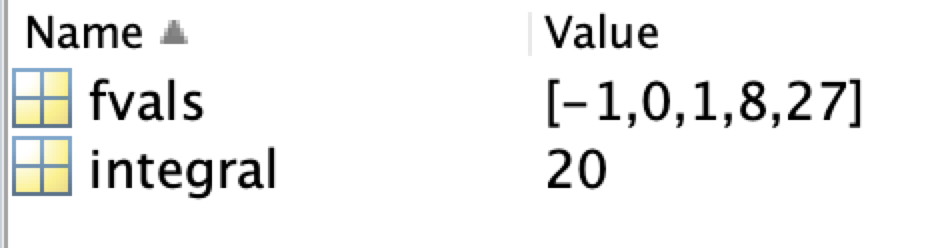
\includegraphics[width=0.7\textwidth]{Figure 8.jpg}
        \caption{\label{fig:fig8}Result of testing the function comp\_simp}
    \end{figure}
    The result it gave to me is true since, $\int_{-1}^{3}x^3\,dx \approx \tfrac{1}{3}(-1 + 4\cdot0 + 2\cdot1 + 4\cdot8 + 27) = 20$ by the composite Simpson's rule
\end{answer}